\section{Вступ}
\todo{Дистрибуція — це діяльність, пов'язана з отриманням продукції, її зберіганням до моменту отримання замовлення і наступної доставки до клієнтів. Управління дистрибуцією включає в себе планування, організацію та контроль.}

\todo{Інформаційні технології в управлінні дистрибуцією вже достатньо розроблені для забезпечення етапів отримання продукції та її збереження, отже зараз найбільш інтенсивно йде розвиток етапу доставки продукції до кінцевих клієнтів. Зокрема розробляються системи автоматизації побудови планових маршрутів руху автотранспорту \cite{art1}, системи керування транспортним парком (TMS) та моніторинг доставок у реальному часі.}

\todo{Велику роль в управлінні дистрибуцією відіграють процеси голосової взаємодії, які зараз активно автоматизуються для підвищення ефективності, збереження ресурсів тощо. Голосова взаємодія поділяється на безпосередню та із залученням інформаційних технологій. Інформаційні технології в цьому контексті можуть слугувати лише засобом забезпечення зв’язку, що саме по собі може давати ефект, але найкращий результат можна отримати, якщо внести певні автоматизації голосової взаємодії.}

\section{Аналіз літературних даних та постановка проблеми}
Японський дослідник з університету Осаки Ішігуро Хіроші з колегами вивчали різні аспекти комунікації та інформаційно-комунікаційних технологій, як, наприклад, використання комунікації з людиноподібними роботами в якості терапевтичної дії для людей похилого віку \cite{Nishio_2015}, аутистів \cite{Kumazaki_2016} чи просто замкнутих у собі людей, педагогічної дії щодо дітей та немовлят \cite{Park_2015} тощо. Зокрема він проводив дослідження голосової комунікації двох людей опосередковано через комп’ютер \cite{Ishiguro_2016}. 

У цьому дослідженні пара спілкувалася на загальні теми, обираючи варіанти своєї репліки із заздалегідь написаного дерева варіантів, свого роду сценарію. Жодному з партнерів не потрібно було нічого промовляти вголос: людині надавався набір з варіантів реплік на вибір, потрібно було лише натиснути на ту з них, яку б вона хотіла  промовити, і ця репліка лунала з динаміків. У залежності від використаної репліки програма вибирала з дерева сценаріїв можливі варіанти відповідей і надавала їх на вибір співрозмовнику. Співрозмовник у свою чергу, чуючи репліку першої людини, обирав свою з наданих варіантів. Це дослідження було спрямоване на подолання сором’язливості при спілкуванні з особами протилежної статі (що є особливо актуальним для Японії). Але такий підхід заздалегідь написаного дерева сценаріїв комунікації можна використовувати і в інших сферах.

У доповіді на світовому психологічному конгресі 2016 проф. Ішігуро демонстрував використання цього сценарного підходу для роботів на виставках та в музеях. Що б уникнути необхідності розпізнавання голосу в шумному середовищі, поряд з експонатом ставиться людиноподібний робот та монітор, на якому показані варіанти запитань. Натискаючи на різні репліки, відвідувач може спілкуватися з роботом по заздалегідь написаному дереву сценаріїв, розпитуючи його про експонат, а робот буде відповідати голосом.

На жаль для управління дистрибуцією постає зворотне завдання — водій має повідомити певну інформацію в систему і при цьому не повинен відволікатися на натискання кнопок на екрані. Тому пряме використання такої технології неможливе. Але застосування підходу описання всіх можливих сценаріїв комунікації в залежності від контексту дозволить знизити кількість інформації, яку треба розпізнати, а отже і підвищити якість.

Наразi існує новий підхід до голосового управління, заснований на теорії несилової взаємодії \cite{Teslia_2010} — рефлекторна система голосового управління \cite{Egorchenkov_2016}. Ідея, покладена в основу цього підходу, полягає в тому, щоб замість переведення голосової інформації в текстову репрезентацію, аналізувати безпосередньо інформаційну складову сказаного, визначаючи, яку з відомих реакцій потрібно виконати. «Традиційні системи розпізнання мови засновані на принципі: „усна мова“ → „репрезентація мови набором лінгвістичних конструкцій“ → „розуміння мови“. На основі теорії несиловой взаємодій може бути запропонована інша модель розпізнання природної мови: „усна мова“ → „розрахунок несилової (інформаційної) взаємодії на реакції“ → „реакція (розуміння чи поведінка)“» \cite{Teslia_2014}.

Така модель розпізнання називається рефлекторною, оскільки побудована за аналогією зі структурою умовного рефлексу, в якому виділяються афектори, центральний компонент та ефектори. Така модель може бути добре поєднана з ідеєю використання дерева сценаріїв, оскільки сценарії також складаються із реакцій, і одиницею моделювання стає не лінгвістична особливість мовлення, а реакція (або команда), яка може бути врахована автоматизованою системою розраховування маршрутів. Тобто, суть цього підходу полягає в тому, щоб перейти до іншої одиниці розпізнання мови. У психології дискурсивного мислення і рефлексивній психології також накопичено досвід аналізу мови, через виокремлення інших одиниць — функціональних висловлювань \cite{Naydonov_2008}.

Оскільки в такій системі не потрібні словники, складні інтелектуальні моделі аналізу тексту та граматики, вони мають низку переваг порівняно з традиційними системами: багатодикторність, варіабельність природної мови, можливість обробки команд офлайн прямо на пристрої, робота в умовах шумів (неконтрольованого акустично середовища), простота алгоритмів та менша складність і ціна реалізації \cite{Teslia_2013}.


\section{Мета та задачі дослідження}
\todo{Метою дослідження є пошук шляхів використання можливостей голосового управління для оптимізації процесів дистрибуції, які не тільки підвищують комфорт водія, а й, фактично, дають змогу автоматизувати певні процеси управління дистрибуцією, покращуючи сервіс та знижуючи витрати.}

\todo{Задача полягає в тому, щоб виокремити підходи, проаналізувати міжнародні здобутки, які вже отримані в різних галузях, для того, щоб побудувати модель їх використання в автоматизації управління дистрибуцією на етапі доставки.}


\section{Матеріали та методи досліджень}
\todo{Для вирішення поставлених завдань було проведено теоретичний аналіз зарубіжних та вітчизняних досліджень, використано наступні методи: логічного узагальнення, аналогій, порівняльного зіставлення та мисленнєвого моделювання.}

\section{\todo{Результати дослідження}}
У результаті аналізу виявлено два найбільш перспективні напрями, поєднання яких дає змогу запропонувати нове принципове рішення і побудувати рефлекторну модель голосової взаємодії в задачах управління дистрибуцією. В основу моделі покладено логічні сценарії взаємодії на тему управління дистрибуцією, які мають враховувати параметри основних причин невідповідності реальної ситуації запланованому маршруту, наприклад, запізнення або відмови обслуговування на точці доставки тощо. Це дає змогу отримати інформацію для прийняття рішення про повернення вантажу на склад, про відміну чи відкладення обслуговування однієї точки доставки, щоб мати можливість встигнути на іншу, більш важливу, про зміну маршруту для об’їзду затору або про утворення нового маршруту з резервною машиною тощо.

Звичайно, абсолютно всі причини та параметри не можуть бути враховані заздалегідь, але проробка і врахування основної типології дозволить приймати базові рішення та вдаватися до безпосереднього зв`язку з диспетчером лише у складних випадках, що розвантажить водія та канали комунікації і дасть змогу підвищити загальну ефективність дистрибуції.

Найбільш ефективним шляхом проробки дерева сценаріїв рефлекторної взаємодії є використання вхідних параметрів вже створеної системи автоматизації дистрибуції, у тому числі автоматичної побудови маршрутів \cite{as6}, яка зараз проходить широку експериментальну апробацію. Інтеграція модулю голосової взаємодії з цією системою буде значно спрощена, що сприятиме отриманню кращого економічного ефекту.

Виходячи з наявної логіки побудови маршрутів, вже зараз можна назвати принципові блоки сценаріїв, які потрібно буде розробити. Першим етапом, на якому можуть виникнути проблеми розбіжності плану та факту, є етап завантаження на складі (якщо, наприклад, буде виявлений неврахований «перегруз» або «недогруз» машини, будуть відсутні необхідні товари чи працівники складу не встигнуть їх вчасно відібрати, або навіть виявиться, що машина не здатна вийти на маршрут (наприклад, не заводитися на морозі)).

\begin{figure}[H]
	{\center
		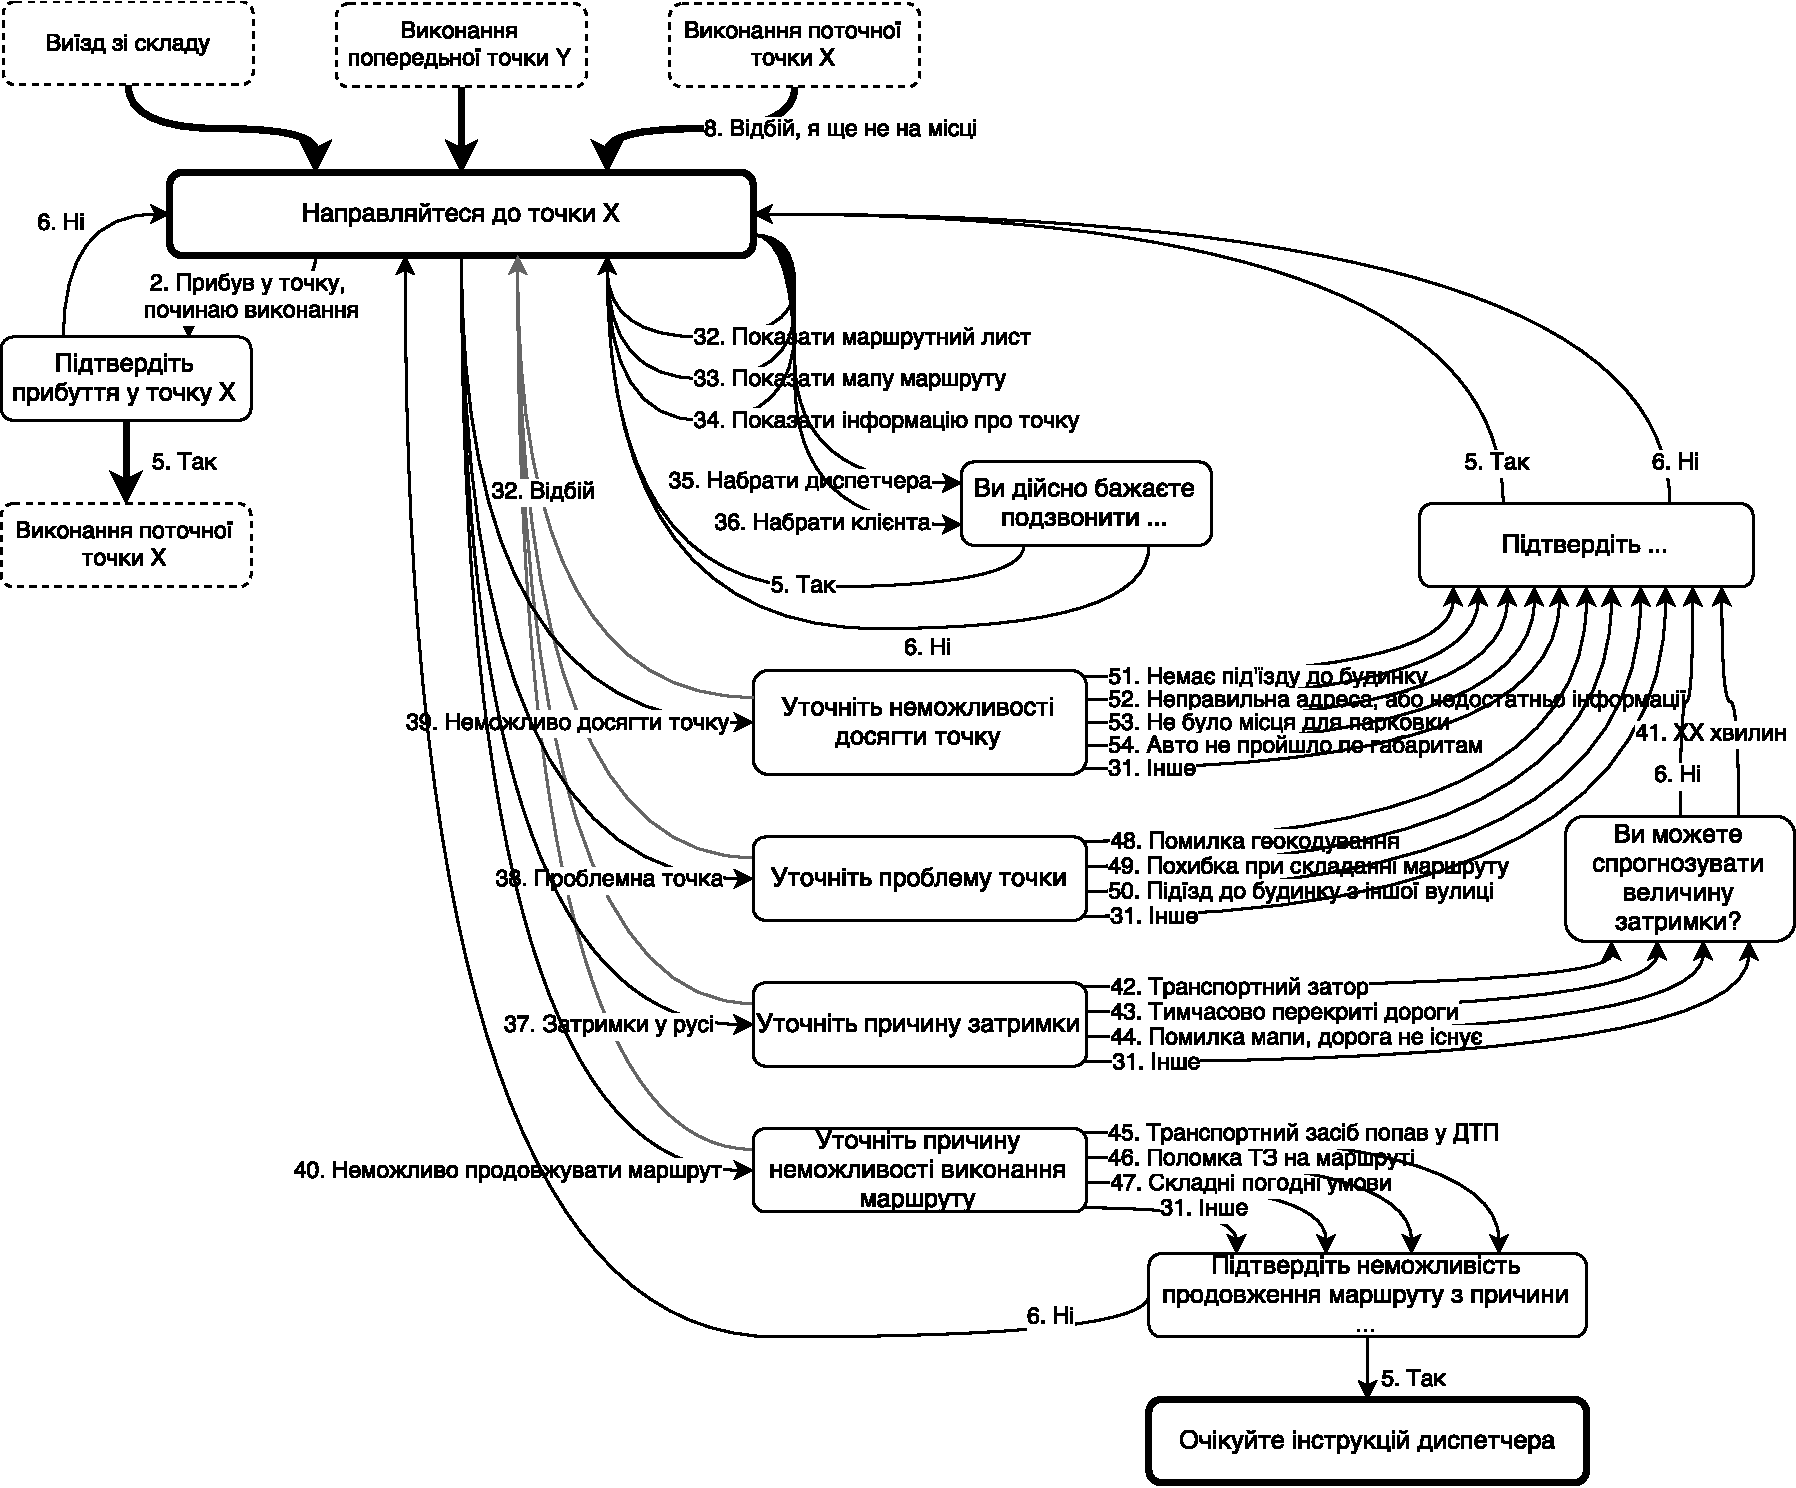
\includegraphics [width=1\linewidth] {11_complete_road_scenario}
		\caption{Частина дерева сценаріїв етапу "дорога"}
		\label{img:11_complete_road_scenario}  }
\end{figure}

Другий етап сценаріїв голосової взаємодії визначають проблеми, які можуть виникнути в дорозі до певної точки доставки, як, наприклад, ремонт в дорозі по маршруту руху або зміни в правилах руху на деяких вулицях, які ще не відбиті в алгоритмах прокладення маршруту (нові заборони поворотів чи односторонній рух), проблеми з автомобілем на дорозі, які призводять до зниження швидкості або відмови в подальшому русі по маршруту, або найбільш розповсюджена проблема заторів на дорогах. 


\begin{figure}[H]
	{\center
		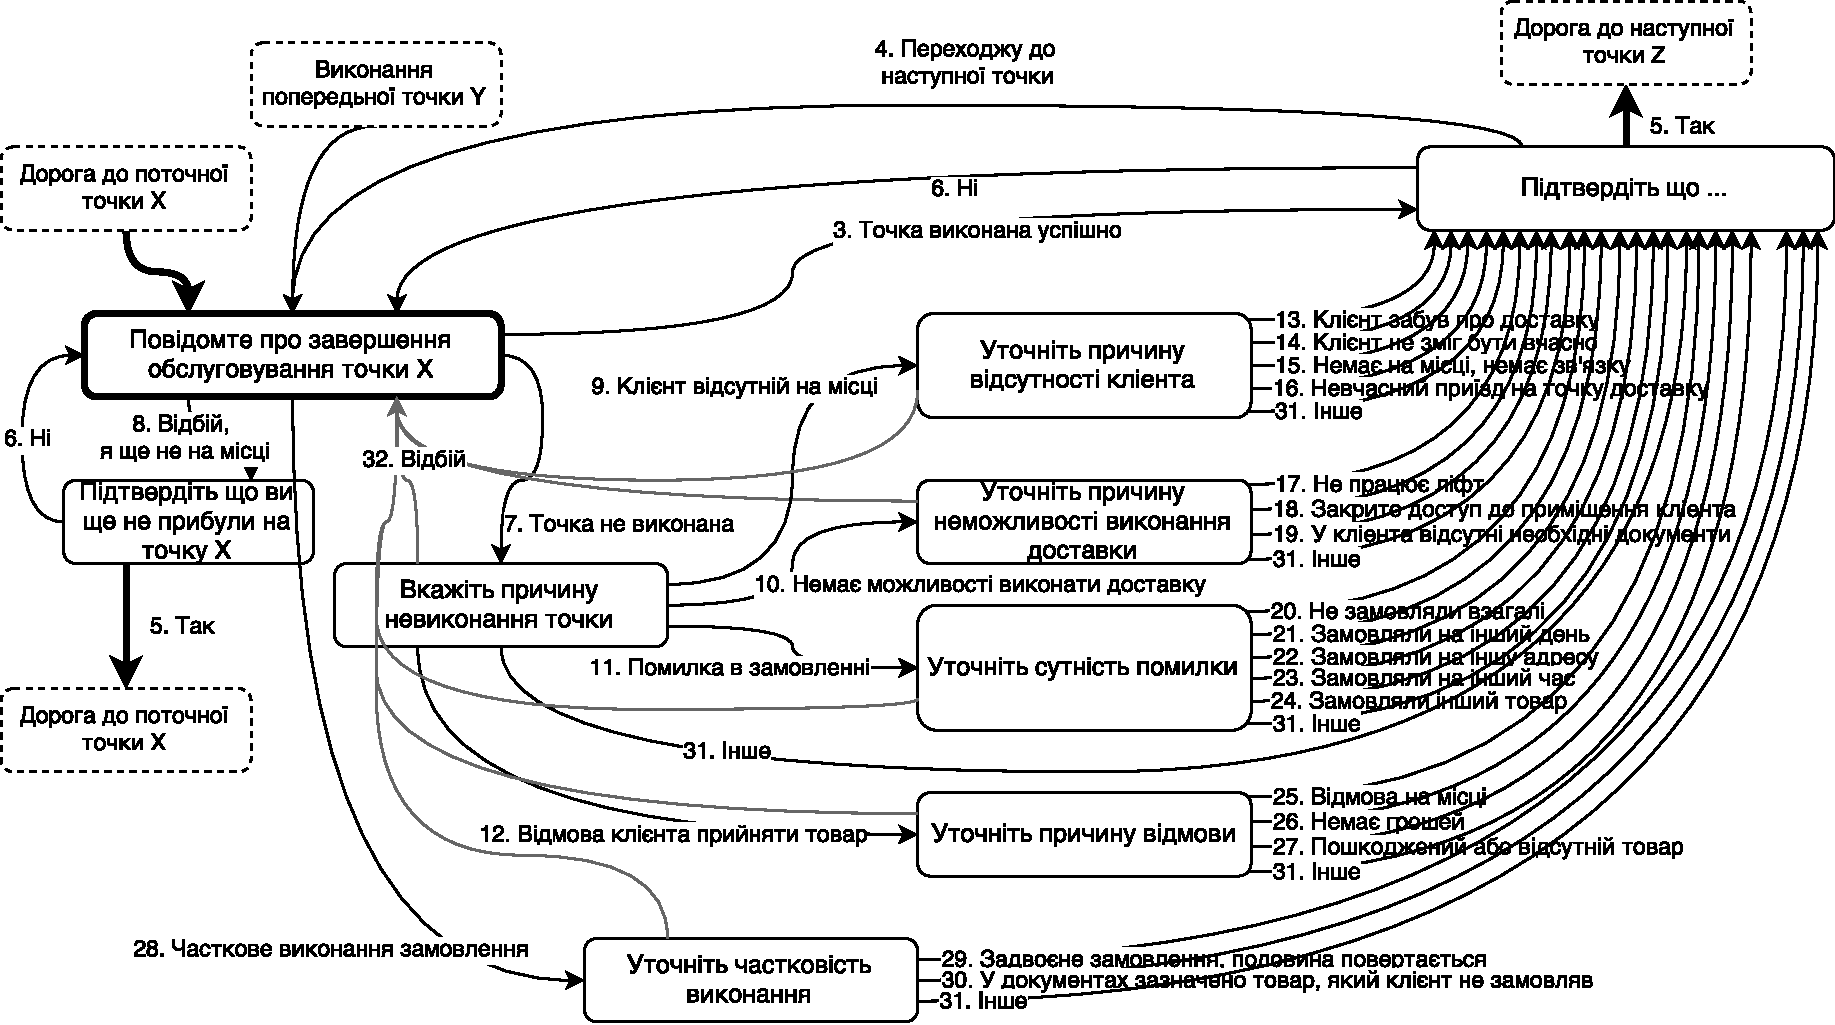
\includegraphics [width=1\linewidth] {09_complete_point_scenario_with_rollback}
		\caption{Частина дерева сценаріїв етапу "точка доставки" з всіма негативними інцидентами та відбоєм із діалогововго режиму}
		\label{img:09_complete_point_scenario_with_rollback}  }
\end{figure}

Третій етап сценаріїв голосової взаємодії викликаний можливими невідповідностями між планом та фактом в обслуговуванні на точці доставки. Це можуть бути як проблеми зі сторони клієнта («нікого немає дома», клієнт не має грошей, клієнт відмовляється від замовлення чи стверджує, що він замовляв щось інше), так і проблеми зі сторони водія (запізнення на точку доставки, тобто не потрапляння в заплановане дозволене часове вікно доступності, пошкодження товару тощо). Найбільш поширеною є ситуація, коли водій проводить в точці доставки більше часу, ніж заплановано, що призводить до проблем на всьому подальшому маршруті.

Ці та інші інциденти на всіх зазначених етапах, що зазначені в моделі на схемі (рис. \ref{img:voice_interaction_schema}), потребують вирішення із залученням диспетчера для вибору найкращої стратегії і мінімізації втрат через проблему. Відповідно дерево сценаріїв голосової взаємодії повинно відбивати всі три етапи та типові відомі проблеми і способи їх розв’язання.

\begin{figure}[H] 
	{\center
		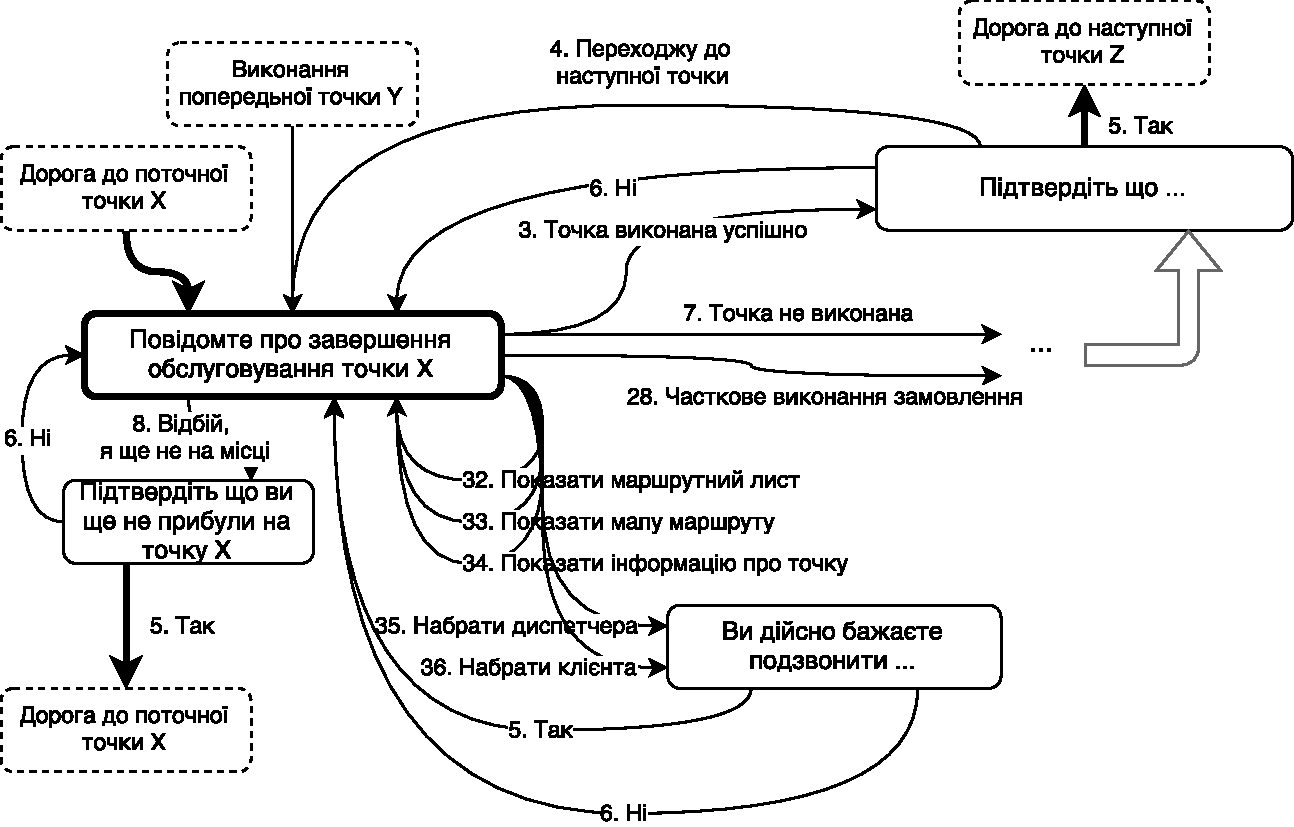
\includegraphics [width=.81\linewidth] {10_point_scenario_with_enchantment}
		\caption{Частина дерева сценаріїв етапу "точка доставки" з додатковими функціями}
		\label{img:10_point_scenario_with_enchantment}  }
\end{figure}

Модель голосової взаємодії суб’єктів дистрибуції може бути зображена на схемі (рис. \ref{img:voice_interaction_schema}). Вона складається з трьох етапів, два останніх з яких, можуть циклічно повторюватися при наявності декількох точок доставки в маршруті. Стрілками позначено процеси голосової взаємодії, які можуть розгортатися на кожному з етапів при невідповідності плану та факту. У верхній та нижній частинах схеми показані принципові типи результатів голосової взаємодії для кожного з суб’єктів (диспетчера та водія). Ця логічна схема визначає принциповий алгоритм побудови деревао сценаріїв голосової взаємодії.

\section{\todo{Обговорення результатів}}
Для представлення дерева сценаріїв найкраще підходить орієнтовний граф, в якому вершини позначають стан системи та діалогові фрази які буде озвучувати система, а ребра --- репліки (стимулів) які можуть бути сприйняті системою в кожній конкретній вершині. Реакція на стимул може привести до переходу між станами, отже орієнтоване ребро проводиться від тієї вершини в якій стимул може буди сприйнятий, до тієї, в який стан система перейде в якості реакції на стимул. Отже множина всіх ребер, що виходять з вершини, позначають перелік стимулів, між якими треба проводити розпізнання для стану, що відповідає цей вершині.

Назва «дерево» сценаріїв використовується як сталий вираз, але реально представити всю необхідну інформацію у вигляді дерева неможливо, адже переходи між станами неминуче приводять до утворення циклів, а отже граф для представлення такої інформації підходить краще.

Нажаль такій схемі недостатньо повноти для представлення всіх можливих варіантів перебігу подій. По перше реакції системи не обмежуються переключенням станів (контекстів) що позначають доступний перелік стимулів та відтворенням діалогових фраз. Основне корисне навантаження системи --- комунікація між водієм і диспетчером та керування процесом доставки,  а отже нам необхідний спосіб представлення інших реакцій на стимули, таких як відправлення певної інформації в диспетчерський центр,  отримання інструкцій з диспетчерського центру,  переключення внутрішніх змінних для можливості повідомити водію контекстно-залежну інформацію про "поточну" точку доставки, тощо.

По друге стимули які можуть викликати певні реакції системи і відповідно переходи між станами не обмежуються голосовими репліками сказаними водієм. Це можуть бути певні події які надійшли з інших джерел інформації, наприклад, команда від диспетчера на зміну маршруту, відміну чи перенос точки доставки, або інформація з внутрішніх джерел данних --- датчиків GPS, роботи двигуна чи відкриття дверей. Використовуючи інформацію з внутрішніх датчиків,  можливо автоматизувати перехід між деякими станами, що підвищить зручність користування системою да ще зменшить кількість необхідних альтернатив для розпізнавання голосових стимулів. 

Отже для повноцінного опису ми маємо такі сутності:

\begin{itemize}
	\item \textbf{Контекст} або \textbf{Стан}, що задає перелік дозволених стимулів, які може сприйняти система в знаходячись в цьому контексті
	\item \textbf{Стимул} або \textbf{Подія} --- певна зовнішня інформація що породжує відповідну реакцію. Стимул може бути голосовою реплікою від водія, командою отриманою від диспетчера або подією породженою інформацією з внутішних датчиків, якщо вони доступні
	\item \textbf{Рекація} системи відповідно до стимулу. Рекцією може бути переключення контексту, відтворення діалогового голосового повідомлення, відправлення певної моніторингової інформації до диспетчерського центру,  переключення внутрішних змінних, тощо. Один стимул може породжувати декілька реакцій різних типів.
\end{itemize}







\section{Висновки}
Були пророблені можливі сценарії взаємодії диспетчера та водія у випадку різних позапланових ситуацій, а також лишив точки розширення для раніше непередбачених варіантів. Запровадження такої автоматизованої системи голосової комунікації між водієм та диспетчером дозволяє спростити для водія повідомлення диспетчеру інформації про позапланові події, які потребують його втручання, коректування маршруту, тощо. Таким чином підвищується швидкість та ефективність отримання диспетчером інформації, відкривається можливість отримати більше інформації чим раніше, чи підвищити її точність, що дозволяє її використовувати для глибшого аналізу та моделювання наступних маршрутів. Крім того робота водія спрощується за рахунок того що він може отримувати голосові поради чи вказівки, в залежності від команд чи даних, що надійшли від диспетчера, або отриманих та обрахованих на самому пристрої у водія
